\chapter{Experiments}
In this chapter experimental results are presented for semi-automated detection of sanitization, authentication and declassification errors in UML state Charts. For three separate problems such as authentication,declassification and sanitization three sample programs selected in C language. Then according to the system these three scenarios are modeled in YAKINDU SCT editor. After this source code file generated and analyzed using static analysis engine. Detailed process how the system works and what is the outcome of the system are given below.

\section{Authentication Scenario}

To understand the authentication scenario a simple example has chosen. The scenario contains a user account creation inside database to access the contents of the database. To access the database contents user have to be authorized by the database administrator or from who is responsible to do the authorization. User creation inside a database now-a-days normally does the database administrator. When database administrator creates the user then user can access the contents of the database otherwise not. In the following Java example the method createUser is used to create a DBAccess object for a database management application.

\begin{lstlisting}
public DBAccess createUser(String userName, String userType,
 String userPassword) {

		DBAccess access = new DBAccess();
		access.setUserName(userName);
		access.setUserType(userType);
		access.setUserPassword(userPassword);	
				
		return access;
}

\end{lstlisting}

However, there is no authentication mechanism to ensure that the user creating this database user account object has the authority to create new user access. Some authentication mechanisms should be used to verify that the user has the authority to create database access objects.
The following Java code includes a boolean variable and method for authenticating a user. If the user has not been authenticated then the createUser will not create the database access object.

\begin{lstlisting}

private boolean isUserAuthentic = false;

// authenticate user,
// if user is authenticated then set variable to true
// otherwise set variable to false
public boolean authenticateUser(String username, String password) {
...
}

public DBAccess createUser(String userName, String userType,
String userPassword) {
			DBAccess access = null;
			
			if (isUserAuthentic) {
			access.setUserName(userName);
			access.setUserType(userType);
			access.setUserPassword(userPassword);
		}
	return access;
}
\end{lstlisting}

To model this kind of scenario in UML statechart considering that for C/C++ application.Figure \ref{authentication_scenario}  represents an authentication scenario. In this scenario a user \emph{A} wants to access a database. At first he/she has to provide his/her user id, password, account number. Then he/she sends request to access database. The database administrator creates a user using his/her id,name and password based on their policy. According to the policy user can either view or access the database or not. If database server doesn't have some secured policy like validation,encryption, decryption or authentication methodology then hacker may easily break the application and receives the confidential information or data from the database server. In Figure \ref{authentication_scenario} depicts a highly secured variable \enquote{char *a} which is initially annotated as H. The annotation is attached with the state named \enquote{char *a}. Annotation are included on the transition from state \enquote{accessDatabase()} to \enquote{char *a}. On the transition annotation is look like this \enquote{//@ @ variable a H False}. The variable \enquote{char *a} passes through a function named authentication. This authentication function is represented as a state in the statechart as like \enquote{void declassification(char *a)}. Annotation of this state \enquote{void declassification(char *a)} is \enquote{/*@ @function authentication
* @parameter a H authenticated @*/} which is attached with the transition from \enquote{char *a} to \enquote{void declassification(char *a)}. This function makes the high secured variable as low by following the policy language. After passing these function the variable \enquote{char *a} is annotated with L and authenticated. Now it can be passed to other system or release information to the authenticated user. While moving from \enquote{void declassification(char *a)} to \enquote{void logIn(char *a)} state there is another annotation which contains annotation \enquote{/*@ @function sink * @parameter a L @*/}. This logIn function is a sink type function and it expects is one of the parameter is low. If the parameter doesn't come through the authentication function then it remains H(High). Then bug should be triggered. Here in this scenario inside the bad\_path() region bug should be triggered because there is no authentication function exist. But if the parameter comes through the authentication function then the parameter will change to L(low). In this scenario inside the good\_path() region there is no bug because it has the authentication function and the variable \enquote{char *a} passes through authentication function.

\begin{figure}[htbp]
	\centering
%	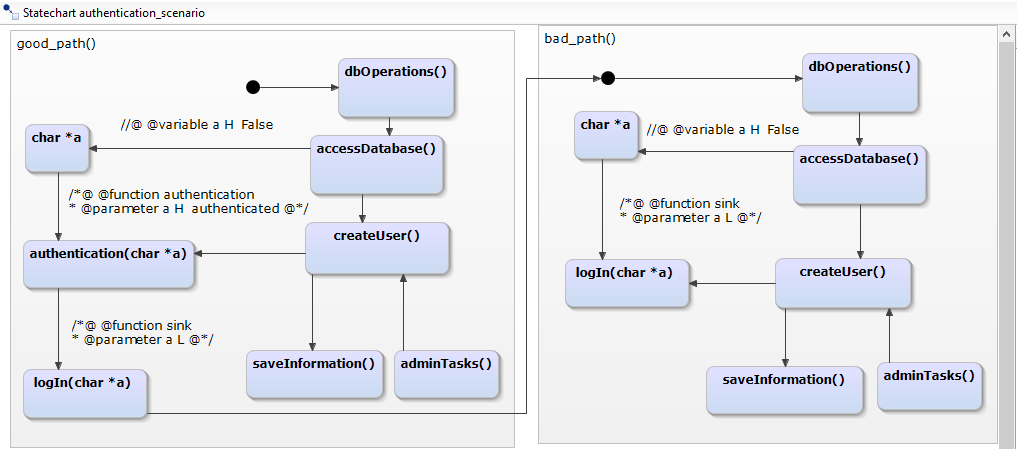
\includegraphics{styles/authentication_scenario.png}
	\makebox[\textwidth]{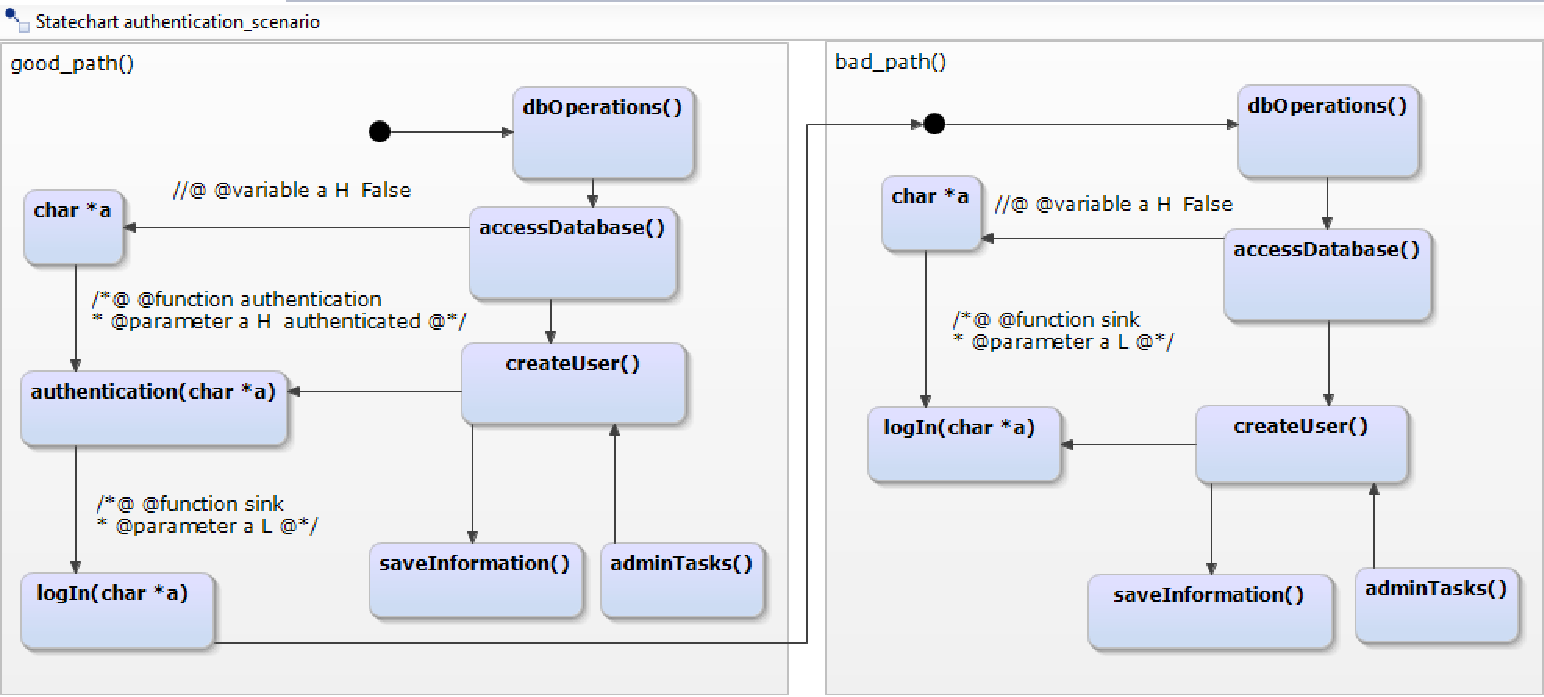
\includegraphics[width=\textwidth,scale=.50]{styles/authentication_scenario.pdf}}
	\label{authentication_scenario}
	\caption{UML Statechart Modeling for Authentication Scenario}
\end{figure}

\section{Declassification Scenario}
 Noninterference is typically
 too strong a property, most programs use some form of declassification to selectively leak high security information when performing a password check or data encryption. Unfortunately, such  a declassification is often expressed as an operation within a given  program, rather than as part of a global policy, making reasoning about the security implications of a policy more difficult. For application programmers need to prevent a range
 of problems, from SQL injection and cross-site scripting, to inadvertent password disclosure and missing access control checks.Adding declassification function is one of the possibility for an application to detect information flow vulnerabilities. It requires few changes to the existing application code and an assertion of functions such as declassification, sanitization and authentication can reuse existing code and data structures. \\
 
 For the declassification scenario, a user \emph{A} wants to access his bank account. Every bank has their own policy to their customer who can access their account information. After giving the password, account number, user name user \emph{A} send his request to the bank server to view the account information. The bank server has his own policy according to their requirements. Through that policy bank server verifies the user \emph{A} may be by following the basic declassification goals according to four axes like what information is released,
 who releases information, where in the system information is released and when information can be released.  \\
 
 Figure \ref{declassification_scenario}  represents a declassification scenario. In this scenario a user \emph{A} wants to access his bank account. At first he/she has to provide his/her user id, password, account number. Then he/she sends request to access his/her account. The bank server has their own policy who can access the account details. According to the policy user can either view his account details or not. If bank server doesn't have some secured policy like encryption, decryption or declassification methodology then hacker may easily break the application and receives the confidential information or data. In Figure \ref{declassification_scenario} depicts a highly secured variable \enquote{char *a} which is initially annotated as H. State \enquote{char *a} has an incoming transition from state \enquote{logInSystem()}. That transition contain annotation like this \enquote{//@ @ variable a H False}. Variable \enquote{char *a} passes through a function named declassification. This declassification function is represented as a state in the statechart as like \enquote{void declassification(char *a)}. This declassification function has an annotation which is like this \enquote{/*@ @function declassification * @parameter a H @*/}. Declassification function makes the high secured variable as low by following the policy language. After passing these function the variable \enquote{char *a} is annotated with L and declassified. Now it can be passed to other function or release information to the verified user. Here in declassification scenario there is a accessAccount function call. The state \enquote{accessAccount(char *a)} expect a parameter which is L(low). If the parameter is low then there would be no bug. But here in case of bad\_path() region there is no declassification method that's why the variable \enquote{char *a} remains H(high). In case of bad\_path() region the state \enquote{accessAccount(char *a)} gets the parameter as H(high) that's why bug should be triggered here. \\
 
 After finishing the modeling of declassification scenario then through the C code generator C code files are generated which consist two files(.c and .h file). Inside those files annotations are exist. Then through static analysis engine named \enquote{smtcodan} analyze the code and detect the information flow vulnerabilities if they exist inside the generated files.
 
\begin{figure}[htbp]
	\centering
%	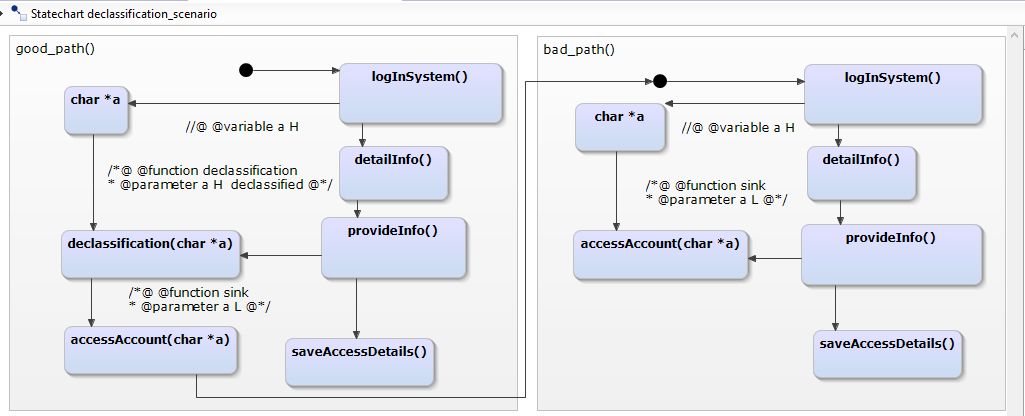
\includegraphics{styles/declassification_scenario.png}
	\makebox[\textwidth]{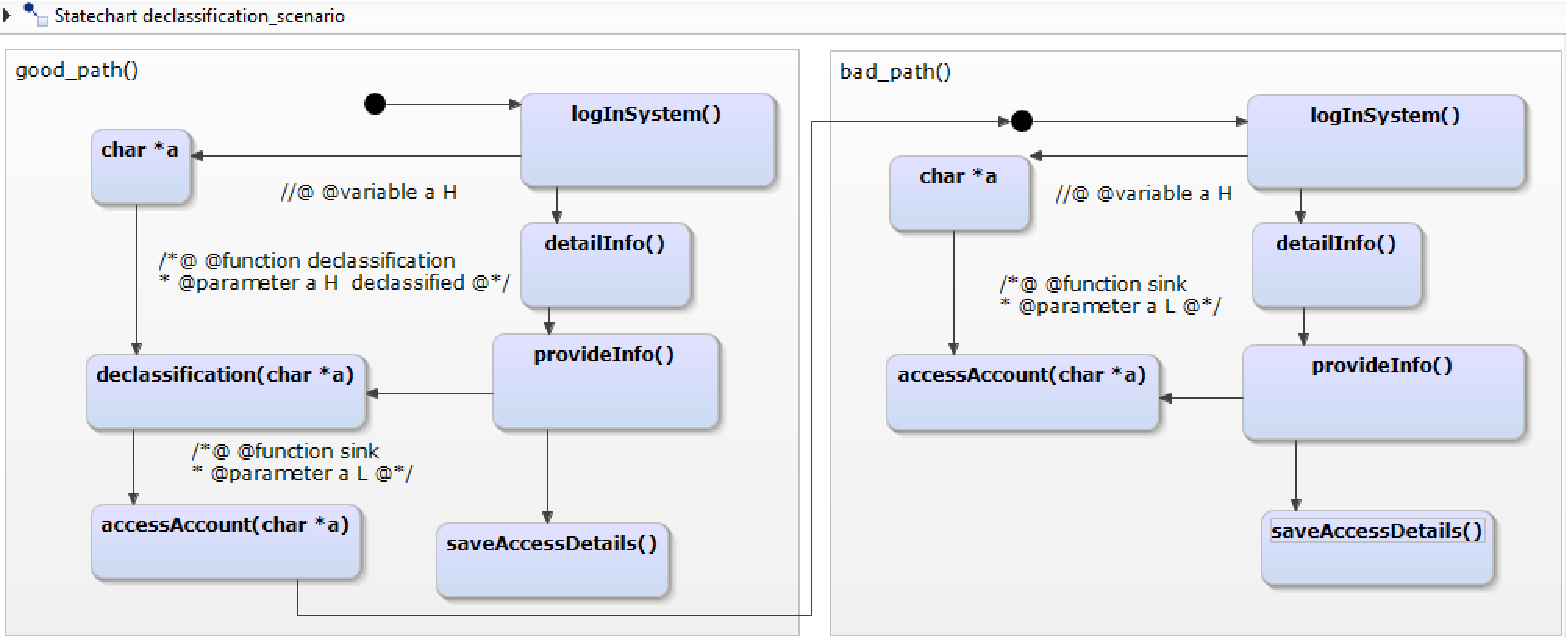
\includegraphics[width=\textwidth,scale=.50]{styles/declassification_scenario.pdf}}
	\label{declassification_scenario}
	\caption{UML Statechart Modeling for Declassification Scenario}
\end{figure}


\section{Sanitization Scenario}
Web applications are often implemented by developers with limited security skills.As a result, they
contain vulnerabilities. Most of these vulnerabilities stem
from the lack of input validation. That is, web applications
use malicious input as part of a sensitive operation, without having properly checked or sanitized the input values
prior to their use.
In the past research on vulnerability analysis has mostly focused on identifying cases in which a web application directly uses external input in critical operations. However,
little research has been performed to analyze the correctness of the sanitization process. Secured web application helps to prevent the bad guys from gaining unauthorized access to your application or website data. It helps you keep your data's integrity and ensures availability as needed. Sql injection and XSS attacks are common attacks now-a-days. to prevent this kind of attacks need to use sanitization methods and validate user input properly.\\
This example code intends to take the name of a user and list the contents of that user's home directory. It is subject to the first variant of OS command injection.Example language is in PHP.

\begin{lstlisting}
	$userName = $_POST["user"];
	$command = 'ls -l /home/' . $userName;
	system($command);
\end{lstlisting} 

The userName variable is not checked for malicious input. An attacker could set the userName variable to an arbitrary OS command such as:
\begin{lstlisting}
;rm -rf /
\end{lstlisting}
Then that would produce a result like this-
\begin{lstlisting}
ls -l /home/;rm -rf /
\end{lstlisting}
Since the semi-colon is a command separator in Unix, the OS would first execute the ls command, then the rm command, deleting the entire file system.\\

The previous example was given for PHP language. In C language here it has been selected that user \enquote{A} wants to access some file from server pc. So, he needs to give the file name. If he wants to access some exe file then bug should be triggered or if he inserts some OS command injection type of statement then bug should be triggered. That's why the user input should pass through a sanitization method to sanitize the input parameter.\\

\begin{figure}[htbp]
	\centering
	%	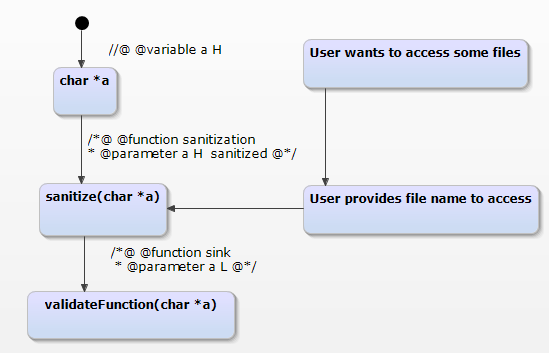
\includegraphics{styles/sanitization_scenario.png}
	\makebox[\textwidth]{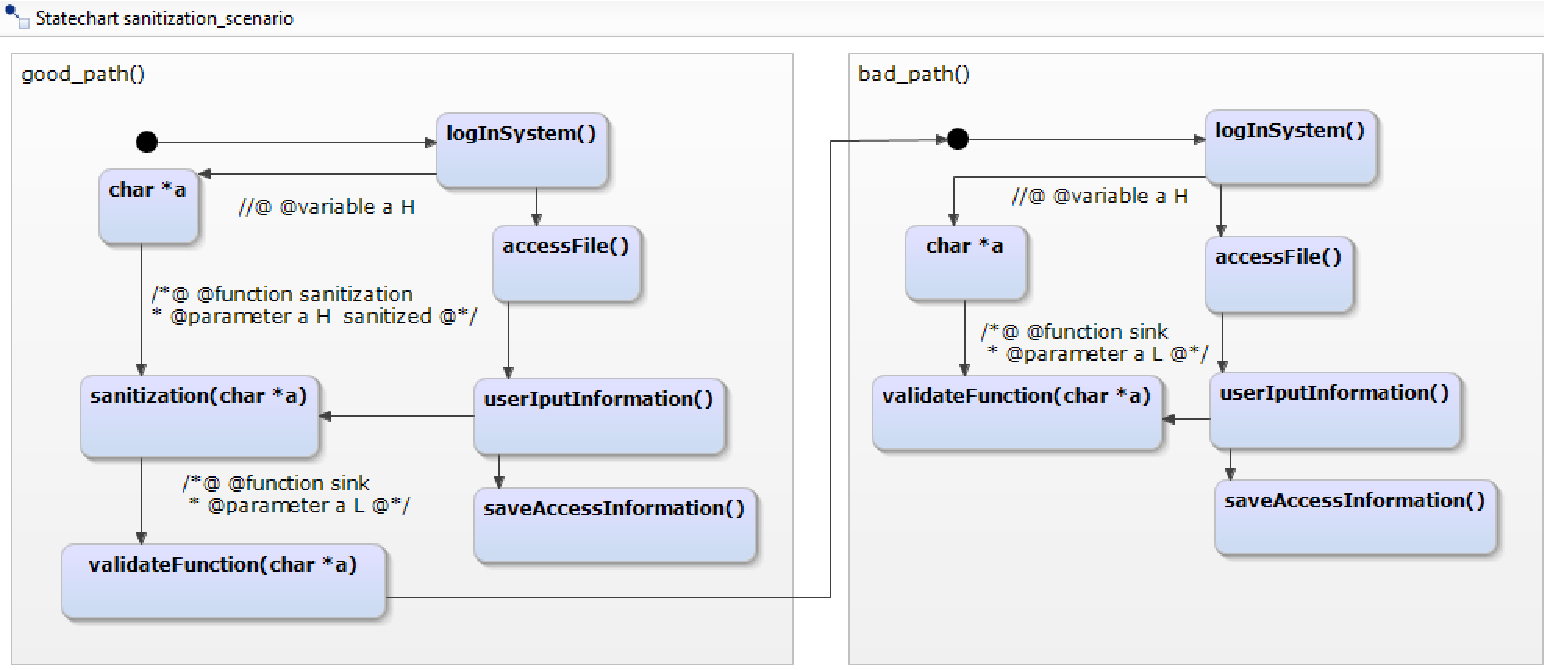
\includegraphics[width=\textwidth,scale=.50]{styles/sanitization_scenario.pdf}}
	\label{sanitization_scenario}
	\caption{UML Statechart Modeling for Sanitization Scenario}
\end{figure}

 Figure \ref{sanitization_scenario} depicts a sanitization scenario. In this scenario a user \emph{A} wants to access file from a server. At first he/she has to provide file name. Then he/she sends request to access his/her desire file. The server has their policy who can access the file. According to the policy if the server has proper sanitization methods then by sanitizing the user input server either allow or disallow the user to access the file. If the server doesn't have some secured policy like encryption, decryption or sanitization methodology then hacker may easily break the application and receives the confidential information or data, even execute the .exe files or may do some OS command injection. In Figure \ref{sanitization_scenario} shows a highly secured variable \enquote{char *a} which is initially annotated as H. It passes through a function named sanitization which also represented as a state named \enquote{void sanitization(char *a)}. This function makes the high secured variable as low by following the policy language. After passing these function the variable \enquote{char *a} is annotated with L and sanitized. Now it can be passed to other function or release information from the system. In good\_path() region there exist sanitization method. So the method make the variable \enquote{char *a} from H(high) to L(Low). So the method validateFunction gets the parameter as L(low). So there would be no bug in good\_path() region. But in bad\_path() region there is no sanitization method. That's why validateFunction get's the parameter as H(high). So there should be bug triggered.



\section{Checkers in Static Analysis Engine}

Static Code Analysis (also known as Source Code Analysis) is usually performed as part of a Code Review (also known as white-box testing) and is carried out at the Implementation phase of a Security Development Lifecycle (SDL). Static Code Analysis commonly refers to the running of Static Code Analysis tools that attempt to highlight possible vulnerabilities within 'static' (non-running) source code by using techniques such as Taint Analysis and Data Flow Analysis.

There are many good reasons to use static code analysis in your project, one of them is thorough analysis of your code, without executing them. Static analysis scans ALL code. If there are vulnerabilities in the distant corners of your application, which are not even used, then also static analysis has a higher probability of finding those vulnerabilities. Second benefit of using static code analysis is you can define your project specific rules, and they will be ensured to follow without any manual intervention. If any team member forget to follow those rules, they will be highlighted by static code analyzer like fortify or find-bugs. Third major benefit of static code analysis is they can find the bug early in development cycle, which means less cost to fix them. All these advantage of static code analyser can be best utilized only if they are part of build process.


A lot of the defects that are present in a program are not visible to the compiler. Static code analysis is a way to find bugs and reduce the defects in a software application.In the 1970's, Stephan Johnson, then at Bell Laboratories, wrote Lint, a tool to examine C
source programs that had compiled without errors and to find bugs that had escaped detection.There are many ways to detect and reduce the number of bugs in a program. For instance in Java, JUnit is a very useful tool for writing tests. Overtime research proved that analyzing the code (especially code reviews) is the best way to eliminate bugs. This is not
always possible because it is very hard to train people and get them together to study and identify problems in programs. Furthermore it is almost impossible to use code inspections on project's complete code base.
Most errors fall into known categories, as people tend to fall into the same traps repeatedly. Therefore a static analyzer or checker is a program written to analyze other programs for flaws. 

Static code analysis, also commonly called white-box testing, looks at applications in non-runtime environment. This method of security testing has distinct advantages in that it can evaluate both web and non-web applications and through advanced modeling, can detect flaws in the software's inputs and outputs that cannot be seen through dynamic web scanning alone. In the past this technique required source code which is not only unpractical as source code often is unavailable but also insufficient.

Some tools are starting to move into the Integrated Development Environment (IDE). For the types of problems that can be detected during the software development phase itself, this is a powerful phase within the development lifecycle to employ such tools, as it provides immediate feedback to the developer on issues they might be introducing into the code during code development itself. This immediate feedback is very useful as compared to finding vulnerabilities much later in the development cycle.The UK Defense Standard 00-55 requires that Static Code Analysis be used on all safety related software in defense equipment.

\textbf{False Positives:}
A static code analysis tool will often produce false positive results where the tool reports a possible vulnerability that in fact is not. This often occurs because the tool cannot be sure of the integrity and security of data as it flows through the application from input to output.

False positive results might be reported when analyzing an application that interacts with closed source components or external systems because without the source code it is impossible to trace the flow of data in the external system and hence ensure the integrity and security of the data.

\textbf{False Negatives:}
The use of static code analysis tools can also result in false negative results where vulnerabilities result but the tool does not report them. This might occur if a new vulnerability is discovered in an external component or if the analysis tool has no knowledge of the runtime environment and whether it is configured securely.

Some tools for static code analysis are given below:
\begin{itemize}
	\item In .NET programming language: .NET Compiler Platform, CodeIt.Right, CodeRush, FxCop, NDepend, StyleCop etc.
	\item In case of C, C++: BLAST, Cppcheck, Clang, Coccinelle, Fluctuat etc.  
	\item For Java: Checkstyle, FindBugs, IntelliJ IDEA, Sonargraph, Soot, Squale etc.
	\item For JavaScript: JSLint, JSHint. 
	\item In Objective-C: Clang.
\end{itemize}

\textbf{Types of Static Code Checkers}: According to the \cite{ref_91_bardas2010static}  static code analyzers come in different flavors, analyzers that work directly on the
program source code and analyzers that work on the compiled byte code. Each type has its own advantages. When analyzing directly the program code, the source code static analyzer checks directly the source program code written by the programmer. Compilers optimize code, and the resulting byte code might not mirror the source.On the other hand, working on byte code is much faster, which is very important on
projects that contain for instance more than one hundred thousand lines of code.

Even though each code checker works differently, most of them share some basic traits.Static checkers read the program and build an abstract representation of it that they are using for matching the error patterns they recognize. On the other hand static checkers
perform some kind of data-flow analysis, trying to infer the possible values that variables might have at certain points in the program. When a program accepts input, there is a possibility that this input can be used to subvert the system. Buffer overflows have been over time hacker's favorite inroad. Nowadays SQL injection seems to have taken the top
place for program sore spots. Therefore data-flow analysis is very important for vulnerability checking. It is essential to be able to trace the input flow from users through the program. There is no code checker that can ever assure developers that a program is correct. Such guarantees aren't possible.In fact, no code checker is complete or sound. A complete code checker would find all errors, while a sound code checker would report only real errors and no false positives.

The percentage of false to true positives indicates if a code checker is suitable for different programs. It is recommended for developers to examine a checker's behavior in their work before committing to it in the whole project. 

Human fallibility is somewhat predictable, but code checkers cannot take all possible bugs into account. Most of the checkers gives programmers the option to define their own rules for the checker to use. In this way, if developers are certain or can predict that they
are particularly prone to some kinds of bugs, they can guard against them by writing custom bug detectors. 

In this research through static code analysis engine named smtcodan was used as the checker to detect the bug in source code files. After the generation of C/C++ code files, those files are included inside the eclipse C/C++ project. This project should be included in the running eclipse instance. Then after running the project as C/C++ code analysis the bug will be detected if any bugs are available inside the project. Figure \ref{bugDetection} depicts the bug reports obtained by running the checkers in parallel on the generated programs. Here for example the sanitization scenario has selected to analyze. At first the generated files are included inside the project named "SantizationScenario". Then the project was run as C/C++ code analysis. Here the circled numbers in Figure \ref{bugDetection} indicate the following: number 1 indicates the analyzed programs (generated programs), number
2 presents bug reports generated by one of the checker for the analyzed programs and number 3 shows the
bug location (line number 69) in source code file scenario3.c by
clicking on the second bug report (Missing Sanitization function Bug
Detected). The bug reports depicted in Figure \ref{bugDetection} with number
2 , confirm that bug is successfully detected and no
false positives and false negatives were generated. Beside the number 2 there also exist more information like file name, line number of the bug location and file path. 

\begin{figure}[htbp]
	\centering
	\makebox[\textwidth]{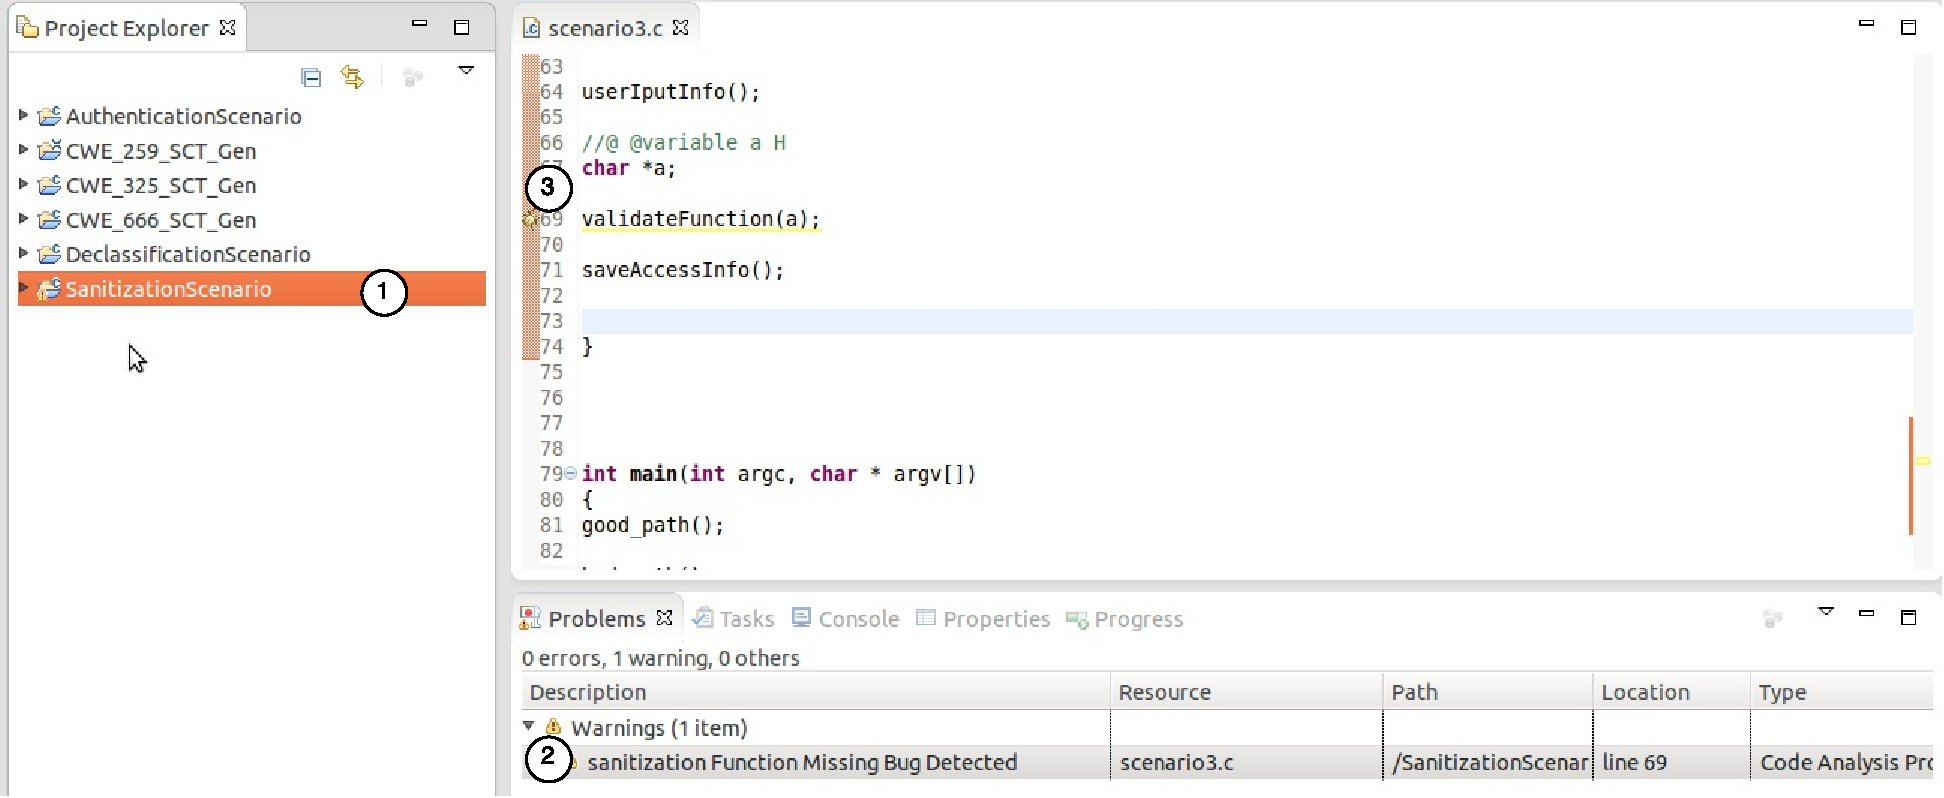
\includegraphics[width=130mm,scale=.50]{styles/bugDetectionDiagram.pdf}}
	\label{bugDetection}
	\caption{Bug Reports in Checker}
\end{figure}

When bug found inside the source file, if user click the bug location then easily can view the bug message.In the figure \ref{bugDetectionWithMessage} it is presented how the message will appear.In the scenario3.c file after clicking the bug symbol in line number 69 the message is appeared as like this sanitization function missing bug detected. 

\begin{figure}[htbp]
	\centering
	\makebox[\textwidth]{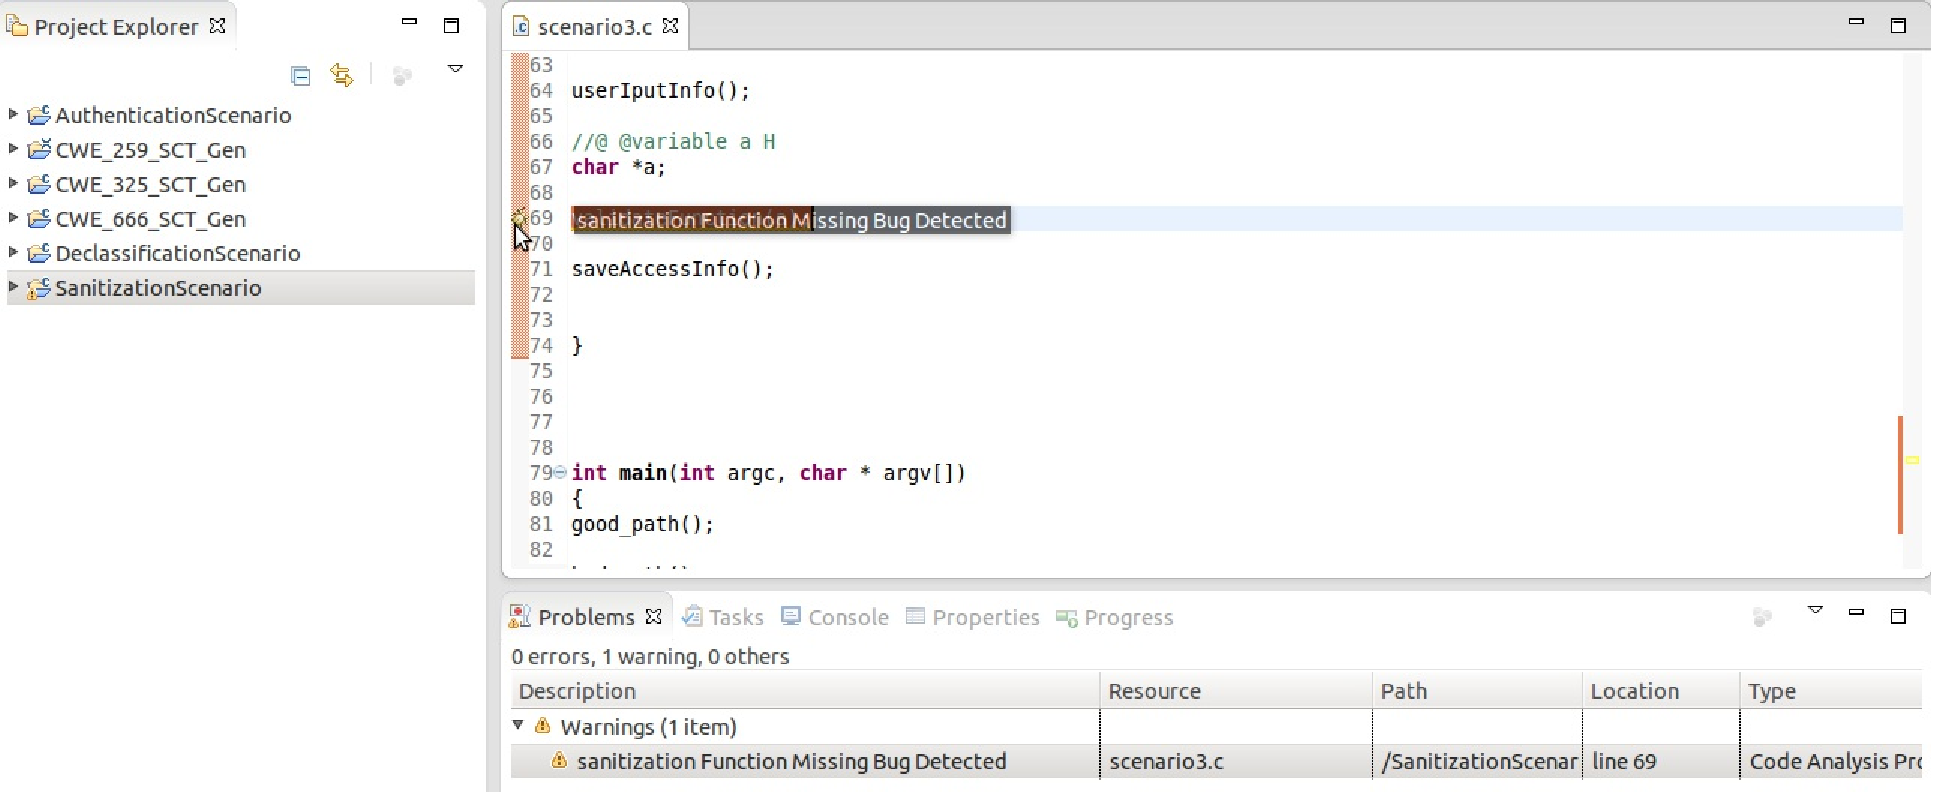
\includegraphics[width=130mm,scale=.50]{styles/bugDetectionWithMessage.pdf}}
	\label{bugDetectionWithMessage}
	\caption{Bug Reports in Checker with Message}
\end{figure}

